% Chapter 2 Support Vector Machine

\chapter{پشینیه پژوهش} \label{ch:2}
\section{ماشین بردار پشتیبان} \label{sec:2:1}
در این بخش، ابتدا ماشین بردار پشتیبان خطی و غیر خطی شرح داده می‌شود. سپس پیشینه پژوهش در زمینه ماشین بردار پشتیبان بررسی می‌گردد.
\subsection{ماشین بردار پشتیبان با حاشیه سخت} \label{sec:2:1:1}
ماشین بردار پشتیبان با هدف جداسازی نمونه‌های دو کلاس در سال 1995 معرفی گردید \cite{vapnik1995}. ایده اصلی این روش یادگیری، بدست آوردن ابرصفحه بهینه‌ای است که از نمونه‌های دو کلاس تا جای ممکن بیشترین فاصله را داشته باشد. به عبارت دیگر، این روش یادگیری حاشیه دو کلاس را بیشینه می‌کند. برای فهم بهتر ایده این روش، فرض کنید مجموعه داده‌ی $T=\{(x_1, y_1),(x_2, y_2) \cdots , (x_m, y_m)\}$ را در اختیار داریم که شامل $m$ تا نمونه آموزشی است. هر نمونه آموزشی $x_{i} \in \mathbb{R}^{n}$ با $n$ ویژگی در فضای ورودی و $y_i \in \{-1,1\}$ برچسب نمونه‌ی $x_i$ می‌باشد. در ساده‌ترین حالت، نمونه‌های دو کلاس در مجموعه داده $T$ با یک ابرصفحه $w^{T}x+b$ بدون خطا دسته‌بندی می‌شود. این حالت مسئله حاشیه سخت\footnote{\lr{Hard margin}}  نامیده می‌شود. شکل \ref{fig:SVM-HM} مسئله حاشیه سخت در روش \lr{SVM} را نشان می‌دهد. (لازم به ذکر است، خطوط نقطه‌چین در شکل ‏\ref{fig:SVM-HM} نشان دهنده حاشیه است.) در این حالت، یک مسئله بهینه‌سازی برای بدست آوردن ابرصفحه باید حل گردد.

\begin{equation}
\begin{gathered} 
\mathop{min}\limits_{w}\frac{1}{2}{{\left\| w \right\|}^{2}} \\
\textrm{\lr{s.t. }} {{y}_{i}}({{w}^T}{{x}_{i}}+b)\ge 1,\forall i
\end{gathered}
\label{eq:1}
\end{equation}

\begin{figure}[!t]
	\centering
	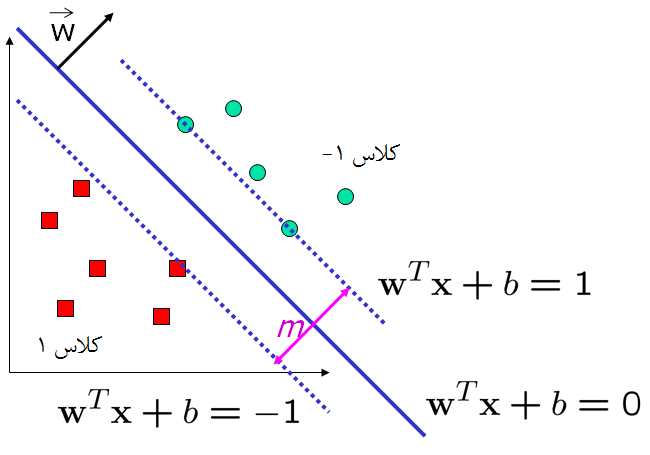
\includegraphics[scale=0.5]{SVM-HardMargin}
	\caption{مسئله حاشیه سخت در ماشین بردار پشتیبان}
	\label{fig:SVM-HM}
\end{figure}

\noindent در رابطه \ref{eq:1}، بردار $w$ مختصات ابرصفحه و $b$ بایاس است. قید این مسئله بهنیه‌سازی بیان می‌کند که تمام نمونه‌های آموزشی باید از ابرصفحه به مقدار 1 یا بیشتر فاصله داشته باشند. به عبارت دیگر، تمام نمونه‌های آموزشی باید روی خط حاشیه یا قبل از آن قرار بگیرند. برای حل کردن مسئله بهینه‌سازی \ref{eq:1} از تابع لاگرانژ\footnote{\lr{Lagrange}}  استفاده می‌شود که در رابطه زیر تعریف شده است. 
\begin{equation}
L(w,b,\alpha )=\frac{1}{2}{{\left\| w \right\|}^{2}}-\sum\limits_{i=1}^{m}{{{\alpha }_{i}}({{y}_{i}}({{w}^{T}}{{x}_{i}}+b)-1})
\label{eq:2}
\end{equation} 
در رابطه \ref{eq:2}، بردار $\alpha$ نشان دهنده ضرایب لاگرانژ است. برای حل کردن رابطه \ref{eq:2}، از تابع لاگرانژ نسبت به $w$ و  $b$ مشتق می‌گیریم.
\begin{align}
\label{eq:3}
\begin{split}
\frac{\partial L}{\partial b}=0&\quad \Rightarrow \quad \sum\limits_{i=1}^{m}{{{\alpha }_{i}}{{y}_{i}}}=0 
\end{split}\\ 
\label{eq:4}
\begin{split}
\frac{\partial L}{\partial w}=0& \quad \Rightarrow \quad w = \sum\limits_{i=1}^{m}{\alpha_{i}y_{i}x_{i}}. 
\end{split} 
\end{align}

با استفاده از اصل دوگانگی لاگرانژ، مسئله اصلی\footnote{\lr{Primal problem}}  در رابطه \ref{eq:1} می‌تواند به مسئله دوگان\footnote{\lr{Dual problem}}  تبدیل شود که حل کردن آن آسان‌تر از مسئله اصلی خواهد بود. با در نظر گرفتن روابط \ref{eq:3} و \ref{eq:4}، مسئله دوگان برای حالت حاشیه سخت به صورت زیر تعریف می‌شود.
\begin{equation}
\begin{split} 
\min\limits_{\alpha} \quad &\frac{1}{2}\sum\limits_{i=1}^{m}{\sum\limits_{j=1}^{m}{{{\alpha }_{i}}{{\alpha }_{j}}{{y}_{i}}{{y}_{j}}x_{i}^{T}{{x}_{j}}-\sum\limits_{k=1}^{m}{{{\alpha }_{k}}}}} \\
\textrm{\lr{s.t. }} \quad &\sum\limits_{i=1}^{m}{\alpha_{i}y_{i}}=0, \\
&\alpha_{i}\ge 0,\text{ }\forall i
\end{split}
\label{eq:5}
\end{equation}
بعد از حل کردن مسئله دوگان \ref{eq:5}، اکثر مقادیر بردار $\alpha$ برابر با صفر خواهد. با این حال ضرایب لاگرانژ  $\alpha_i$ متناظر با نمونه‌های $x_i$ بزرگتر از صفر خواهد بود، اگر معادله زیر برقرار باشد.
\begin{equation}
{{y}_{i}}({{w}^{T}}{{x}_{i}}+b)=1
\label{eq:6}
\end{equation}
\indent نمونه‌های  که رابطه \ref{eq:6} برای آن‌ها برقرار باشد، به اصطلاح بردار پشتیبان\footnote{\lr{Suppor Vector (SV)}}  نامیده می‌شود. ضرایب لاگرانژ متناظر با بردار‌های پشتیبان بزرگ‌تر از صفر است. همچنین این بردارها روی حاشیه قرار می‌گیرند. بردار $w$  و بایاس  $b$ از طریق رابطه  بدست می‌آید.
\begin{equation}
\begin{split}
w &= \sum\limits_{i=1}^{m}{\alpha_{i}y_{i}x_{i}} \\
b &= y_{i}-{w}^{T}{x}_{i}
\end{split}
\label{eq:7}
\end{equation}
یک نمونه جدید یا تست بر اساس تابع تصمیم در رابطه زیر به یکی از کلاس‌های 1 و 1- تعلق می‌گیرد.
\begin{equation}
D(x)=sign({{w}^{T}}x+b) = sign(\sum\limits_{i=1}^{m}{\alpha_{i}y_{i}x_{i}^{T}} x + b)
\label{eq:8}
\end{equation}
\indent در مسئله حاشیه سخت، فرض گرفته می‌شود که تمام نمونه‌های دو کلاس به صورت خطی جدا پذیر هستند. با این حال در دنیای واقعی داده‌ها اغلب به صورت خطی جدا پذیر نیستند. در حالتی که داده‌ها به صورتی خطی جداپذیر نیستند، مسئله حاشیه نرم\footnote{\lr{Soft margin}}  در ماشین بردار پشتیبان مطرح شده است.

\subsection{ماشین بردار پشتیبان با حاشیه نرم} \label{sec:2:1:2}
در این حالت اجازه خطا در دسته‌بندی نمونه‌ها داده می‌شود. به عبارت دیگر، با معرفی متغیر کمکی\footnote{\lr{Slack variable}} $\xi$ ، تاثیر بعضی از نمونه‌های آموزشی در ایجاد حاشیه و ابرصفحه کم می‌شود. برای درک بهتر، مسئله حاشیه نرم در ماشین بردار پشتیبان در شکل \ref{fig:SVM-SM}‏ نشان داده شده است. در حالت حاشیه نرم، برای بدست آوردن ابرصفحه مسئله بهینه‌سازی به صورت زیر تعریف می‌شود.

\begin{figure}[!t]
	\centering
	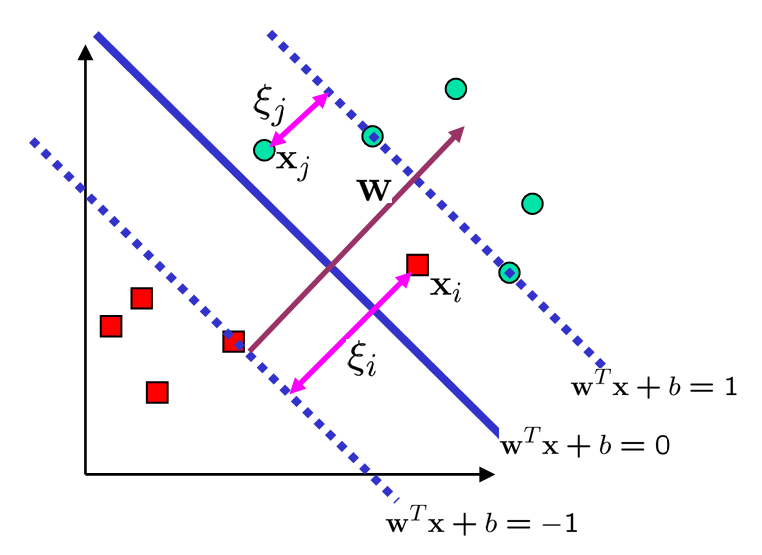
\includegraphics[scale=0.5]{SVM-SoftMargin}
	\caption{مسئله حاشیه نرم در ماشین بردار پشتیبان}
	\label{fig:SVM-SM}
\end{figure}

\begin{equation}
\begin{split}
\min_{w} \quad &\frac{1}{2}{{\left\| w \right\|}^{2}}+C\sum\limits_{i=1}^{n}{{{\xi }_{i}}} \\
\textrm{\lr{s.t. }}  \quad &{{y}_{i}}({{w}^{T}}{{x}_{i}}+b)\text{ }+{{\xi }_{i}}\ge 1,\forall i
\end{split}
\label{eq:9}
\end{equation}
در رابطه \ref{eq:9}، متغیر $\xi _{i}\ge 0$ خطای متناظر برای هر نمونه  $x_i$ است. پارامتر $C$ بیانگر تعادل بین بیشینه کردن حاشیه و خطای دسته‌بندی است. مقدار این پارامتر قبل از آموزش دسته‌بند باید مشخص گردد. مانند مسئله حاشیه سخت، برای حل کردن مسئله اصلی  از تابع لاگرانژ استفاده می‌شود که در رابطه زیر تعریف شده است.
\begin{equation}
L(w,b,\xi, \alpha, \beta )=\frac{1}{2}{{\left\| w \right\|}^{2}} + C\sum\limits_{i=1}^{m}{{{\xi }_{i}}}  -\sum\limits_{i=1}^{m}{{{\alpha }_{i}}({{y}_{i}}({{w}^{T}}{{x}_{i}}+b)-1 + \xi_{i} }) - \sum\limits_{i=1}^{m}{\beta_{i}\xi_{i}}
\label{eq:10}
\end{equation}
در رابطه \ref{eq:10}، بردار $\alpha$  و $\beta$  ضرایب لاگرانژ هستند. برای حل کردن رابطه \ref{eq:10}، نسبت به  $w$، $b$ و $\xi$  مشتق می‌گیریم.
\begin{align}
\label{eq:11}
\begin{split}
\frac{\partial L}{\partial b}&=0\quad \Rightarrow \quad \sum\limits_{i=1}^{m}{{{\alpha }_{i}}{{y}_{i}}}=0
\end{split}\\ 
\label{eq:12}
\begin{split}
\frac{\partial L}{\partial w}&=0 \quad \Rightarrow \quad w = \sum\limits_{i=1}^{m}{\alpha_{i}y_{i}x_{i}}.
\end{split}\\
\label{eq:13}
\begin{split}
\frac{\partial L}{\partial \xi}&=0 \quad \Rightarrow \quad \alpha_{i} + \beta_{i} = C
\end{split}  
\end{align}
با در نظر گرفتن روابط بالا، مسئله دوگان برای حالت حاشیه نرم به صورت زیر تعریف می‌شود.
\begin{equation}
\begin{split} 
\min\limits_{\alpha} \quad &\frac{1}{2}\sum\limits_{i=1}^{m}{\sum\limits_{j=1}^{m}{{{\alpha }_{i}}{{\alpha }_{j}}{{y}_{i}}{{y}_{j}}x_{i}^{T}{{x}_{j}}-\sum\limits_{k=1}^{m}{{{\alpha }_{k}}}}} \\
\textrm{\lr{s.t. }} \quad &\sum\limits_{i=1}^{m}{\alpha_{i}y_{i}}=0, \\
&0 \le \alpha_{i}\le C,\text{ }\forall i
\end{split}
\label{eq:14}
\end{equation}
\indent راه حل مسئله \ref{eq:14} شبیه به مسئله \ref{eq:5} در حالت حاشیه سخت است. با این تفاوت که برای ضرایب لاگرانژ یک حد بین صفر تا پارامتر  تعریف شده است. پارامتر  انعطاف‌پذیری دسته‌بند را افزایش می‌دهد. مقدار این پارامتر با داشتن دانش قبلی از مسئله و یا جستجوی شبکه‌ای تعیین می‌شود. همانطور که در شکل ‏\ref{fig:SVM-SM} نشان داده شده است، بردارهای پشتیبان لزوما روی خط حاشیه قرار ندارند. در مسئله حاشیه نرم، تابع تصمیم مشابه حالت حاشیه سخت به صورت زیر تعریف می‌شود.
\begin{equation}
D(x)=sign({{w}^{T}}x+b) = sign(\sum\limits_{i \in S}{\alpha_{i}y_{i}x_{i}^{T}} x + b)
\label{eq:15}
\end{equation}
در رابطه \ref{eq:15}، مجموعه $S$ نشان دهنده بردارهای پشتیبان است.

\subsection{ماشین بردار پشتیبان با هسته غیر خطی}\label{sec:2:1:3}
در مسائل حاشیه سخت و نرم، فرض گرفته می‌شود که نمونه‌ها در فضای ورودی به صورت خطی جدا پذیر هستند. با این حال در مواردی که نمونه‌ها به صورت خطی جدا پذیر نیستند، نمونه‌ها $x_i$ به فضای ویژگی\footnote{\lr{Feature space}}  با ابعاد بیشتر با تکنیک حقه‌ی هسته\footnote{\lr{Kernel trick}}  نگاشت می‌شود. در این فضا، ماشین بردار پشتیبان یک ابرصفحه جدا کننده بهینه برای جداسازی نمونه‌ها پیدا می‌کند. شکل \ref{fig:SVM-Ker} تکنیک حقه‌ی هسته را نشان می‌دهد.

\begin{figure}[!t]
	\centering
	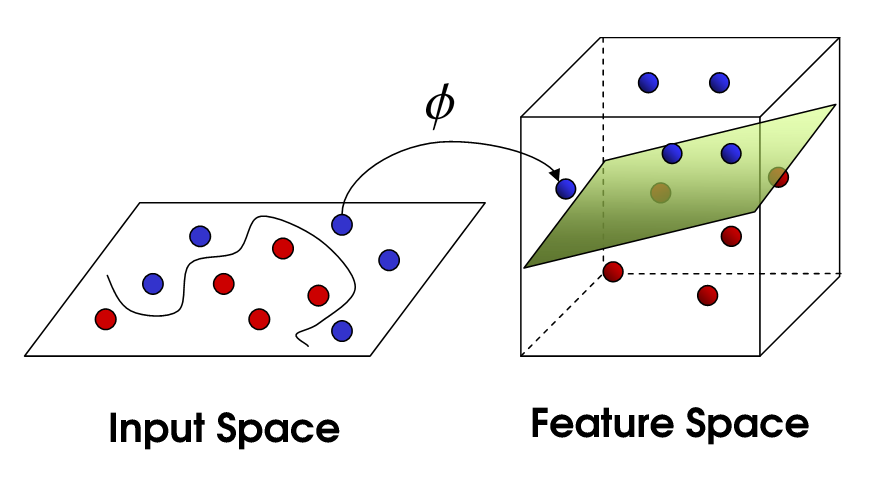
\includegraphics[scale=0.4]{SVM-Kernel}
	\caption{نگاشت نمونه‌ها با تکنیک حقه‌ی هسته}
	\label{fig:SVM-Ker}
\end{figure}

در نسخه غیر خطی ماشین بردار پشتیبان، مسئله \ref{eq:14} به صورت زیر تعریف می‌شود.
\begin{equation}
\begin{split} 
\min\limits_{\alpha} \quad &\frac{1}{2}\sum\limits_{i=1}^{m}{\sum\limits_{j=1}^{m}{{{\alpha }_{i}}{{\alpha }_{j}}{{y}_{i}}{{y}_{j}}K(x_{i},{{x}_{j}})-\sum\limits_{k=1}^{m}{{{\alpha }_{k}}}}} \\
\textrm{\lr{s.t. }} \quad &\sum\limits_{i=1}^{m}{\alpha_{i}y_{i}}=0, \\
&0 \le \alpha_{i}\le C,\text{ }\forall i
\end{split}
\label{eq:16}
\end{equation}
در رابطه \ref{eq:16}‏، تابع هسته  $K({{x}_{i}},{{x}_{j}})$ نمونه‌ها را به فضای ویژگی نگاشت می‌کند. تابع‌های هسته متداول شامل  \lr{RBF}\footnote{\lr{Radial basis function (RBF)}}، چند جمله‌ای و سیگموئید\footnote{\lr{Sigmoid}}  هستند. تابع تصمیم در نسخه غیر خطی به صورت زیر تعریف می‌شود.
\begin{equation}
D(x)= sign(\sum\limits_{i \in S}{\alpha_{i}y_{i}}K(x_{i}, x) + b)
\label{eq:17}
\end{equation}

\subsection{پیشینه پژوهش در ماشین بردار پشتیبان}\label{sec:2:1:4}
ماشین بردار پشتیبان بنیان ریاضی قوی‌ای دارد و دارای قدرت تعمیم‌پذیری بالایی است. از این رو در مسائل مختلف انند تشخیص آریتمی‌های قلبی \cite{nasiri2009}، شناسایی نفوذ به شبکه‌های کامپیوتری \cite{raman2017}، دسته‌بندی متن\cite{lee2012} و شناسایی 
هرزنامه \cite{zoubi2018} مورد استفاده قرار گرفته است. با این حال ماشین بردار پشتیبان نقاط ضعفی نیز دارد که مهم‌ترین آن‌ها عبارتند از:
\begin{enumerate}
	\item ماشین بردار پشتیبان برای بدست آوردن ابرصفحه بهینه یک مسئله بهینه‌سازی از نوع برنامه‌ریزی درجه دو حل می‌کند. مرتبه زمانی حل کردن چنین مسئله‌ای برابر با   $\mathcal{O}({{m}^{3}})$ است.  $m$ تعداد نمونه‌های آموزشی می‌باشد. این مرتبه زمانی، آموزش روش ماشین بردار پشتیبان را برای مجموعه داده‌های بزرگ به طور قابل توجه‌ای کند می‌کند.
	\item در روش \lr{SVM}، بردارهای پشتیبان نقش مهمی در ایجاد مدل دارند. در صورتی که این بردارها از نمونه‌های پرت یا نویزی باشد، دقت و تعمیم‌پذیری مدل خروجی کاهش می‌یابد. در نتیجه روش \lr{SVM} به نمونه‌های پرت و نویزی حساس است.
	\item چنانچه نمونه‌های یک کلاس از کلاس دیگر بسیار بیشتر باشد (مجموعه داده نامتوازن باشد.)، مدل ایجاد شده توسط  \lr{SVM} به سمت کلاس اکثریت گرایش پیدا می‌کند. در نتیجه مدل در تشخیص کلاس اقلیت ناتوان است.
\end{enumerate}

\indent در دو دهه اخیر، روش‌های یادگیری جدیدی مبتنی \lr{SVM} ارائه شده است که برخی از آن‌ها نقاط ضعف بالا را حل می‌کند. در سال 1999، ماشین بردار پشتیبان کمترین مربعات\footnote{\lr{Least squares support vector machines  (LS-SVM)}}  ارائه شد \cite{suykens1999}. در این روش قید در مسئله بهینه‌سازی از نامساوی به مساوی تبدیل شده است. بطوریکه به جای حل کردن مسئله بهینه‌سازی از نوع برنامه‌ریزی درجه دو، دستگاه معادلات خطی حل می‌گردد. در نتیجه سرعت یادگیری برای مجموعه داده‌های بزرگ بسیار بیشتر می‌شود و نقطه ضعف مورد اول تا حد زیادی حل شده است.

در سال 2001، ماشین بردار پشتیبان مبتنی بر مفهوم نزدیکی\footnote{\lr{Proximal Support Vector Machine (PSVM)}}  (\lr{PSVM}) ارائه شد \cite{mang2001}. در این روش دو ابرصفحه موازی برای دسته‌بندی نمونه‌ها ایجاد می‌شود. در سال 2002، ماشین بردار پشتیبان فازی\footnote{\lr{Fuzzy Support Vector Machine (FSVM)}}  (\lr{FSVM}) \cite{lin2002} ارائه گردید. در این روش به هر یک از نمونه‌های هر دو کلاس، تعلق فازی داده می‌شود. بطوریکه اثر نمونه‌های نویزی و پرت در ایجاد مدل خروجی کم خواهد شد. در سال 2006، ماشین بردار پشتیبان با رویکرد مقدار ویژه تعمیم یافته\footnote{\lr{Generalized Eigenvalue Proximal Support Vector Machine (GEPSVM)}}  (\lr{GEPSVM}) ارائه شد \cite{mang2006}. برخلاف روش \lr{PSVM}، این روش دو ابرصفحه غیر موازی ایجاد می‌کند که هر یک از این ابرصفحه‌ها به نمونه‌های کلاس خود نزدیک است و از نمونه‌های کلاس مقابل تا جای ممکن فاصله می‌گیرد. همچنین روش \lr{PSVM} بر روی مسئله \lr{XOR} عملکرد بهتری نسبت به روش \lr{SVM} اصلی دارد.

در سال 2007، ماشین بردار پشتیبان دو قلو\footnote{\lr{Twin Support Vector Machine (TSVM)}}  (\lr{TSVM}) با هدف بهبود پیچیدگی زمانی \lr{SVM} ارائه گردید \cite{jayadeva2007}. ایده اصلی این روش یادگیری، بدست آوردن دو ابرصفحه غیر موازی است. بطوریکه هر ابرصفحه غیر موازی به نمونه‌های کلاس خود نزدیک است و نمونه‌های کلاس مقابل دور می‌شود. دو مسئله بهینه‌سازی کوچک از نوع برنامه‌ریزی درجه دو برای بدست آوردن این دو ابرصفحه غیر موازی حل می‌گردد. در حالی‌که در روش \lr{SVM} یک مسئله بهینه‌سازی بزرگ حل می‌شود. در نتیجه، روش ماشین بردار پشتیبان دو قلو در تئوری 4 برابر سریعتر از روش \lr{SVM} است. در بخش ‏2-2 ماشین بردار پشتیبان دو قلو و پیشینه پژوهش آن به طور کامل بررسی می‌شود.

در سال‌های اخیر نیز، روش‌های جدید مبتنی بر \lr{SVM} ارائه شده است. در سال 2018، می‌توان به روش یادگیری برخط مبتنی بر بدترین نمونه‌ی نقض‌کننده\footnote{\lr{Online Learning Algorithm using Worst-Violators (OLLAWV)}}  اشاره کرد \cite{melki2018}. این الگوریتم بر اساس گرادیان نزولی تصادفی\footnote{\lr{Stochastic Gradient Descent (SGD)}}  طراحی شده است و مسئله اصلی در روش \lr{SVM} را به جای مسئله دوگان حل می‌کند. مزایای این روش، دقت بهتر، سرعت یادگیری بیشتر برای مجموعه داده‌های بزرگ و همچنین مدل خلوت\footnote{\lr{Sparse}}  می‌باشد.

\section{ماشین بردار پشتیبان دو قلو}\label{sec:2:2}
در این بخش، ابتدا نسخه خطی ماشین بردار پشتیبان دو قلو شرح داده می شود. سپس نسخه غیر خطی این روش توضیح داده شده و در آخر پیشینه پژوهش آن و روش‌های مبتنی بر \lr{TSVM} بررسی می‌شود.

\subsection{ماشین بردار پشتیبان دو قلو خطی}\label{sec:2:2:1}
ایده اصلی روش \lr{TSVM}، ایجاد دو ابرصفحه غیر موازی است \cite{jayadeva2007}. بطوریکه هر ابرصفحه غیر موازی از نمونه‌های کلاس خود کمترین فاصله را دارد و از نمونه‌های کلاس مقابل حداکثر فاصله ممکن را خواهد داشت. برای تشریح بهتر این روش، یک مسئله دسته‌بندی دوکلاسه با $m_1$  نمونه آموزشی کلاس مثبت و  $m_2$ نمونه آموزشی کلاس منفی را در نظر می‌گیریم. همچنین فرض می‌کنیم که ماتریس   $A\in {{\mathbb{R}}^{{{m}_{1}}\times n}}$ بیانگر نمونه‌های کلاس مثبت و ماتریس  $B\in {{\mathbb{R}}^{{{m}_{2}}\times n}}$ بیانگر نمونه‌های کلاس منفی است. روش \lr{TSVM} در حالت خطی به دنبال دو ابرصفحه غیر موازی در فضای  ${{\mathbb{R}}^{n}}$ است که در رابطه زیر تعریف شده است.
\begin{equation}
{{x}^T}{{w}_{1}}+{{b}_{1}}=0 \quad \textrm{\lr{and }} \quad {{x}^T}{{w}_{2}}+{{b}_{2}}=0
\label{eq:18}
\end{equation}
در رابطه \ref{eq:18}،  ${{w}^{(1)}},{{w}^{(2)}}\in {{\mathbb{R}}^{n}}$ نشان دهنده مختصات دو ابرصفحه و  ${{b}^{(1)}},{{b}^{(2)}}\in {\mathbb{R}}$ نشان دهنده بایاس است. شکل ‏2 4 تفسیر هندسی روش ماشین بردار پشتیبان دوقلو خطی را نشان می‌دهد. در روش \lr{TSVM}، دو مسئله بهینه‌سازی از نوع برنامه‌ریزی درجه دو برای بدست آوردن دو ابرصفحه غیر موازی به صورت زیر تعریف می‌شود.
\begin{figure}[!t]
	\centering
	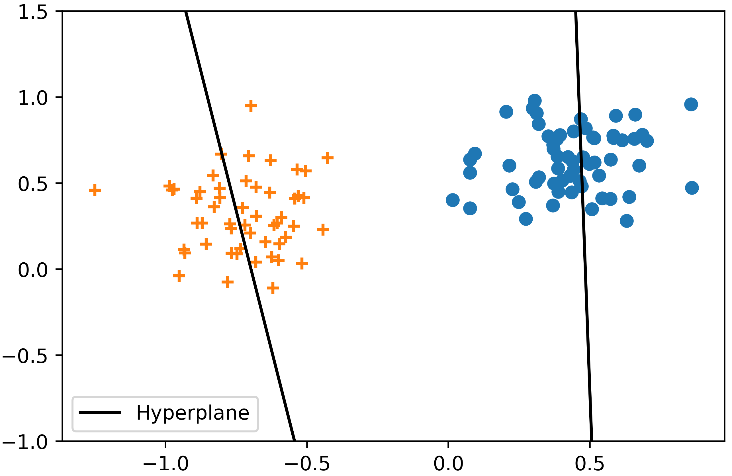
\includegraphics[scale=0.75]{TSVM-idea}
	\caption{تفسیر هندسی روش ماشین بردار پشتیبان دو قلو خطی}
	\label{fig:TSVM-idea}
\end{figure}
\begin{align}
\label{eq:19}
\begin{split}
\underset{{{w}_{(1)}},{{b}_{(1)}}}{\mathop{min}}\,\qquad  & \frac{1}{2}{{\left\| A{{w}^{(1)}}+{{e}_{1}}{{b}^{(1)}} \right\|}^{2}}+{{C}_{1}}e_{2}^{T}{{y}_{2}}  \\
\text{\lr{s.t.}} \qquad  & -(B{{w}^{(1)}}+{{e}_{2}}{{b}^{(1)}})+{{y}_{2}}\ge {{e}_{2}}\text{ },{{y}_{2}}\ge 0  
\end{split} \\
%\end{equation}
%\begin{equation}
\label{eq:20}
\begin{split}
\underset{{{w}_{(2)}},{{b}_{(2)}}}{\mathop{min}}\,\qquad  & \frac{1}{2}{{\left\| B{{w}^{(2)}}+{{e}_{2}}{{b}^{(2)}} \right\|}^{2}}+{{C}_{2}}e_{1}^{T}{{y}_{1}}  \\
\text{\lr{s.t.}} \qquad  & (A{{w}^{(2)}}+{{e}_{1}}{{b}^{(2)}})+{{y}_{1}}\ge {{e}_{1}}\text{ },{{y}_{1}}\ge 0  
\end{split}
\end{align}
\bigbreak
در روابط \ref{eq:19} و \ref{eq:20}،  $C_1$ و $C_2$  پارامترهای خطا،  $e_1$ و  $e_2$ بردار با درایه‌های یک در ابعاد متناسب،  $y_1$ و $y_2$  متغیر کمکی هستند. لازم به ذکر است که تعداد نمونه‌ها در مسائل بهینه‌سازی روش \lr{TSVM} تقریبا برابر با $m/2$ در نظر گرفته می‌شود. با این حال در روش \lr{SVM}، در قید مسئله بهینه‌سازی تمام نمونه‌های آموزشی نقش دارند. بنابراین زمان اجرای روش \lr{TSVM} از روش \lr{SVM} حدود 4 برابر سریع‌تر است که زیر نشان داده شده است.
\begin{equation}
\Big[({{m}^{3}})/(2\times {{(\frac{m}{2})}^{3}})\Big] = 4.
\label{eq:21}
\end{equation}

مانند روش \lr{SVM}، برای حل کردن مسائل بهینه‌سازی \ref{eq:19}، از تابع لاگرانژ استفاده می‌کنیم.
\begin{equation}
\begin{split}
L(w_{1},b_{1},y_{2}, \alpha, \beta )= &\frac{1}{2}(A{{w}^{(1)}}+{{e}_{1}}{{b}^{(1)}})^{T}(A{{w}^{(1)}}+{{e}_{1}}{{b}^{(1)}}) + {{C}_{1}}e_{2}^{T}y_{2} \\
&-\alpha^{T}(-(Bw^{(1)}+e_{2}b^{(1)})+y_{2} - e_{2}) - \beta^{T}y_{2}
\end{split}
\label{eq:22}
\end{equation}

در رابطه \ref{eq:22}، $\alpha=(\alpha_{1}, \alpha_{2}, \dots,\alpha_{m_{2}})^{T}$ و $\beta=(\beta_{1}, \beta_{2}, \dots,\beta_{m_{2}})^{T}$ بردارهای ضرایب لاگرانژ هستند.  با مشتق‌گیری از رابطه \ref{eq:22}، شرایط \lr{KKT}\footnote{\lr{Karush-Kuhn-Tucker}}  زیر برقرار می‌شود.
\begin{align}
\label{eq:23}
\begin{split}
A^{T}(A{{w}^{(1)}}+{{e}_{1}}{{b}^{(1)}}) + B^{T}\alpha = 0.
\end{split} \\
\label{eq:24}
\begin{split}
e_{1}^{T}(A{{w}^{(1)}}+{{e}_{1}}{{b}^{(1)}}) + e_{2}^{T}\alpha = 0.
\end{split}\\
\label{eq:25}
\begin{split}
C_{1}e_{2} - \alpha - \beta = 0.
\end{split} 
\end{align}
با توجه اینکه $\beta \ge 0$، از رابطه \ref{eq:25} خواهیم داشت:
\begin{equation}
0 \le \alpha \le {C}_{1}
\label{eq:26}
\end{equation}

سپس با ترکیب کردن \ref{eq:23} و \ref{eq:24}، رابطه زیر بدست می‌آید.
\begin{equation}
[A^{T}\ e^{T}_{1}][A\ e_{1}][w^{(1)}\ b^{(1)}]^{T} + [B^{T}\ e^{T}_{2}]\alpha = 0.
\label{eq:27}
\end{equation}

با تعریف کردن ماتریس $H$ و $G$ به صورت $H=[A\text{ }e]$ و $G=[B\text{ }e]$، رابطه \ref{eq:27} به صورت زیر بازنویسی می‌شود.
\begin{equation}
\left[ \begin{aligned}
& {{w}^{(1)}} \\
& {{b}^{(1)}} \\
\end{aligned} \right]= -{{({{H}^{T}}H)}^{-1}}{{G}^{T}}\alpha
\label{eq:28}
\end{equation}

برای جلوگیری از شرایط ماتریس منفرد\footnote{\lr{Singular}}  در ماتریس $H^{T}H$، یک عدد ثابت بسیار کوچک  $\varepsilon > 0, \varepsilon I$ به عناصر قطر این ماتریس اضافه می‌شود. بنابراین دستگاه معادلات در رابطه \ref{eq:28} به صورت زیر تغییر می‌یابد.
\begin{equation}
\left[ \begin{aligned}
& {{w}^{(1)}} \\
& {{b}^{(1)}} \\
\end{aligned}\right]= -{{({{H}^{T}}H + \varepsilon I)}^{-1}}{{G}^{T}}\alpha
\label{eq:29}
\end{equation}

با توجه به شرایط \lr{KKT} و مسئله اصلی \ref{eq:19}، مسئله دوگان برای \ref{eq:19} به صورت زیر تعریف می‌گردد.
\begin{equation}
\begin{split}
\mathop{{ min}}\limits_{\alpha} \qquad & \frac{1}{2}{{\alpha }^{T}}G{{({{H}^{T}}H)}^{-1}}{{G}^{T}}\alpha -e_{2}^{T}\alpha  \\
\textrm{\lr{s.t. }} \qquad & 0{{e}_{2}}\le \alpha \le {{C}_{1}}{{e}_{2}}
\end{split}
\label{eq:30}
\end{equation}

مشابه راه حل کلاس مثبت، مسئله دوگان برای کلاس منفی \ref{eq:20} به صورت زیر تعریف می‌شود.
\begin{equation}
\begin{split}
\mathop{{ min}}\limits_{\alpha} \qquad & \frac{1}{2}{{\alpha }^{T}}G{{({{H}^{T}}H)}^{-1}}{{G}^{T}}\alpha -e_{2}^{T}\alpha  \\
\textrm{\lr{s.t. }} \qquad & 0{{e}_{2}}\le \alpha \le {{C}_{1}}{{e}_{2}}
\end{split}
\label{eq:31}
\end{equation}

بعد از حل کردن مسئله دوگان \ref{eq:31}، ابرصفحه کلاس منفی از طریق رابطه زیر بدست می‌آید.
\begin{equation}
\left[ \begin{aligned}
& {{w}^{(2)}} \\
& {{b}^{(2)}} \\
\end{aligned}\right]= {{({{G}^{T}}G)}^{-1}}{{H}^{T}}\beta
\label{eq:32}
\end{equation}

در نسخه خطی روش \lr{TSVM}، برای بدست آوردن مدل خروجی دو گام محاسباتی وجود دارد که عبارتند از:
\begin{enumerate}
	\item ضرایب لاگرانژ $\alpha$  و $\beta$  به ترتیب با حل کردن مسائل دوگان \ref{eq:31} و \ref{eq:32} بدست می‌آید. مرتبه زمانی این گام برابر با$\mathcal{O}({1/4{m}^{3}})$  می‌باشد.
	\item	دو دستگاه معادلات خطی در روابط   \ref{eq:29} و \ref{eq:32} باید حل گردد. در این گام، معکوس ماتریس های  $H^{T}H$ و  $G^{T}G$ باید محاسبه شود. ابعاد این دو ماتریس برابر $(n + 1) \times (n + 1)$  است. بطوریکه   $n$ بسیار کوچکتر از تعداد نمونه‌های   کلاس مثبت و منفی می‌باشد.
\end{enumerate}

بعد از بدست آمدن دو ابرصفحه غیرموازی \ref{eq:18}، داده جدید با تابع تصمیم زیر به یکی از کلاس‌های مثبت یا منفی تعلق می‌گیرد.
\begin{equation}
\underset{j=1,2}{\mathop{arg\min }}\,\text{ } \left| {{x}^{T}}{{w}^{(j)}}+{{b}^{(j)}} \right|
\label{eq:33}
\end{equation}

\subsection{ماشین بردار پشتیبان دو قلو غیر خطی}\label{sec:2:2:2}
مسائل یادگیری ماشین در دنیای واقعی غالبا به صورت خطی جدا پذیر نیستند. روش \lr{TSVM} برای جدا سازی مسائل غیر خطی، نمونه‌ها را به فضای ویژگی با ابعاد بالاتر نگاشت می‌کند. بدین منظور دو ابرسطح\footnote{\lr{Hypersurface}}  به صورت زیر تعریف می‌شود.
\begin{equation}
K({{x}^{T}},~{{C}^{T}}){{u}^{\left( 1 \right)}}+{{b}^{\left( 1 \right)}}=0 \text{\lr{ and }} K({{x}^{T}},~{{C}^{T}}){{u}^{\left( 2 \right)}}+{{b}^{\left( 2 \right)}}=0
\label{eq:34}
\end{equation}

در رابطه \ref{eq:34}، ماتریس $C$ برابر با  $C=~\left[ A \  B \right]^{T}$ است و $K$ تابع هسته دلخواه می‌باشد. در نسخه غیر خطی، مسائل بهینه‌سازی اصلی برای کلاس مثبت و منفی به ترتیب در روابط \ref{eq:35} و \ref{eq:36} تعریف شده است. 
\begin{equation}
\begin{split}
\mathop{{ min}}\limits_{u^{(1)} ,b^{(1)}} \qquad & \frac{1}{2}{{\left\| K(A, C^{T}){{u}^{(1)}}+{{e}_{1}}{{b}^{(1)}} \right\|}^{2}}+{{C}_{1}}e_{2}^{T}y_{2} \\
\textrm{\lr{s.t. }} \qquad & -(K(B, C^{T}){{u}^{(1)}}+{{e}_{2}}{{b}^{(1)}})+ y_{2} \ge {{e}_{2}}\text{ },y_{2}\ge 0
\end{split}
\label{eq:35}
\end{equation}
\begin{equation}
\begin{split}
\mathop{{ min}}\limits_{u^{(2)} ,b^{(2)}} \qquad & \frac{1}{2}{{\left\| K(B, C^{T}){{u}^{(2)}}+{{e}_{2}}{{b}^{(2)}} \right\|}^{2}}+{{C}_{2}}e_{1}^{T}y_{1} \\
\textrm{\lr{s.t. }} \qquad & (K(A, C^{T}){{u}^{(2)}}+{{e}_{1}}{{b}^{(2)}})+ y_{1} \ge {{e}_{1}}\text{ },y_{1}\ge 0
\end{split}
\label{eq:36}
\end{equation}

تابع لاگرانژ برای مسئله اصلی در رابطه \ref{eq:35} به صورت زیر تعریف می‌شود.
\begin{equation}
\begin{split}
L(u_{1},b_{1},y_{2}, \alpha, \beta )= & \frac{1}{2}{{\left\| K(A, C^{T}){{u}^{(1)}}+{{e}_{1}}{{b}^{(1)}} \right\|}^{2}} + {{C}_{1}}e_{2}^{T}y_{2} \\
&-\alpha^{T}(-(K(B, C^{T})u^{(1)}+e_{2}b^{(1)})+y_{2} - e_{2}) - \beta^{T}y_{2}
\end{split}
\label{eq:37}
\end{equation}

مشابه نسخه خطی، شرایط \lr{KKT} برای رابطه \ref{eq:37} زیر تعریف شده است.
\begin{align}
\label{eq:38}
\begin{split}
K(A, C^{T})^{T}(K(A,C^{T}){{u}^{(1)}}+{{e}_{1}}{{b}^{(1)}}) + K(B, C^{T})^{T}\alpha = 0.
\end{split} \\
\label{eq:39}
\begin{split}
e_{1}^{T}(K(A,C^{T}){{u}^{(1)}}+{{e}_{1}}{{b}^{(1)}}) + e_{2}^{T}\alpha = 0.
\end{split}\\
\label{eq:40}
\begin{split}
C_{1}e_{2} - \alpha - \beta = 0.
\end{split} 
\end{align}

با ترکیب کردن روابط \ref{eq:38} و \ref{eq:39}، رابطه زیر بدست می‌آید.
\begin{equation}
[K(A,C^{T})^{T}\ e^{T}_{1}][K(A,C^{T})\ e_{1}][u^{(1)}\ b^{(1)}]^{T} + [K(B, C^{T})\ e^{T}_{2}]\alpha = 0.
\label{eq:41}
\end{equation}

با تعریف کردن ماتریس $S$ و $R$  به صورت $S=[K(A,C^{T})\text{ }e_{1}]$ و $R=[K(B,C^{T})\text{ }e_{2}]$ ، رابطه \ref{eq:41} به صورت بازنویسی می‌شود.
\begin{equation}
\left[ \begin{aligned}
& {{u}^{(1)}} \\
& {{b}^{(1)}} \\
\end{aligned}\right]= -{{({{S}^{T}}S)}^{-1}}{{R}^{T}}\alpha
\label{eq:42}
\end{equation}

با توجه به شرایط \lr{KKT} و مسئله اصلی \ref{eq:35}، مسئله دوگان برای بدست آوردن ضریب لاگرانژ $\alpha$ به صورت زیر تعریف می‌شود.
\begin{equation}
\begin{split}
\mathop{{ min}}\limits_{\alpha} \qquad & \frac{1}{2}{{\alpha }^{T}}R{{({{S}^{T}}S)}^{-1}}{{R}^{T}}\alpha -e_{2}^{T}\alpha  \\
\textrm{\lr{s.t. }} \qquad & 0{{e}_{2}}\le \alpha \le {{C}_{1}}{{e}_{2}}
\end{split}
\label{eq:43}
\end{equation}

به طرز مشابه‌ای، مسئله دوگان مسئله اصلی \ref{eq:36} در رابطه زیر تعریف شده است.
\begin{equation}
\begin{split}
\mathop{{ min}}\limits_{\beta} \qquad & \frac{1}{2}{{\beta }^{T}}S{{({{R}^{T}}R)}^{-1}}{{S}^{T}}\beta -e_{1}^{T}\beta  \\
\textrm{\lr{s.t. }} \qquad & 0{{e}_{1}}\le \beta \le {{C}_{2}}{{e}_{1}}
\end{split}
\label{eq:44}
\end{equation}

بعد از حل کردن مسئله دوگان و بدست آمدن ضرایب لاگرانژ $\beta$، ابرسطح کلاس منفی از طریق رابطه زیر بدست می‌آید.
\begin{equation}
\left[ \begin{aligned}
& {{u}^{(2)}} \\
& {{b}^{(2)}} \\
\end{aligned}\right]= {{({{R}^{T}}R)}^{-1}}{{S}^{T}}\alpha
\label{eq:45}
\end{equation}

بعد از حل کردن مسائل دوگان \ref{eq:43} و \ref{eq:44}، مشابه نسخه خطی یک نمونه جدید به کلاس مثبت یا منفی نسبت داده می‌شود. به عبارت دیگر، براساس فاصله عمودی نمونه جدید از دو ابرسطح، کلاس آن مشخص می‌گردد. 

برخلاف نسخه خطی، حل کردن روابط \ref{eq:42} و \ref{eq:45} نیاز به محاسبه معکوس ماتریس در ابعاد  $m  \times m$  دارد. بطوریکه  $m$ برابر با کل نمونه‌های آموزشی است. زمانی که مجموعه داده‌ها بزرگ باشد، بدست آوردن مدل غیر خطی بسیار زمان‌بر می‌شود. تکنیک هسته‌ی مستطیلی\footnote{\lr{Rectangular kernel}} \cite{mang2001} برای کاهش ابعاد مسئله و بهبود محاسبه استفاده می‌شود.

\subsection{پیشینه پژوهش در ماشین بردار پشتیبان دو قلو}\label{sec:2:2:3}
روش \lr{TSVM} نسبت به روش \lr{SVM} دو نقطه قوت مهم دارد که عبارتند از:
\begin{enumerate}
	\item 	حساسیت کمتری به مجموعه داده‌های نامتوزان دارد و دقت آن روی این گونه داده‌ها بیشتر است.
	\item دو مسئله دوگان کوچکتر برای بدست آوردن مدل خروجی حل می شود. به عبارتی هر مسئله دوگان فقط شامل نمونه‌های یک کلاس است. در حالی که در \lr{SVM} تمام نمونه‌ها در مسئله دوگان نقش دارند.
\end{enumerate}

با این حال ماشین بردار پشتیبان دوقلو نقاط ضعفی نیز دارد. در دهه اخیر، دسته‌بند‌هایی مبتنی بر \lr{TSVM} ارائه شده است که نقاط ضعف \lr{TSVM} را حل می‌کند \cite{ding2014,ding2017,huang2018}. در ادامه برخی از گسترش‌های مهم روش \lr{TSVM} در زیربخش‌های جداگانه توضیح داده شده است. در آخر سایر روش‌های مبتنی بر \lr{TSVM} در یک زیربخش به طور خلاصه معرفی شده است.

\subsubsection{ماشین بردار پشتیبان دو قلو کمترین مربعات}\label{sec:2:2:3:1}
روش \lr{TSVM} اصلی دو مسئله دوگان برای ایجاد مدل خروجی حل می‌کند. بطوریکه سرعت آموزش و ایجاد مدل در \lr{TSVM} برای مجموعه داده‌های بزرگ به طور قابل توجه‌ای کاهش می‌یابد. به منظور افزایش سرعت آموزش، ماشین بردار پشتیبان دو قلو کمترین مربعات\footnote{\lr{Least Squares Twin Support Vector Machine (LS-TSVM)}}  (\lr{LS-TSVM})  در سال 2009 ارائه گردید \cite{kumar2009}. در این روش، برای بدست آوردن دو ابرصفحه غیر موازی دو مسئله بهینه‌سازی به صورت زیر تعریف می‌شود.
\begin{equation}
\begin{split}
 \underset{{{w}^{(1)}},{{b}^{(1)}},y}{\mathop{Min}} \qquad &\frac{1}{2}{{\left\| A{{w}^{(1)}}+{{e}_{1}}{{b}^{(1)}} \right\|}^{2}}+\frac{{{C}_{1}}}{2}e_{2}^{T}y \\ 
\textrm{\lr{s.t. }} \qquad & -(B{{w}^{(1)}}+{{e}_{2}}{{b}^{(1)}})+y={{e}_{2}}
\end{split}
\label{eq:46}
\end{equation}
\begin{equation}
\begin{split}
\underset{{{w}^{(2)}},{{b}^{(2)}},y}{\mathop{Min}} \qquad & \frac{1}{2}{{\left\| B{{w}^{(2)}}+{{e}_{2}}{{b}^{(2)}} \right\|}^{2}}+\frac{{{C}_{2}}}{2}e_{1}^{T}y \\ 
\textrm{\lr{s.t. }} \qquad & (A{{w}^{(2)}}+{{e}_{1}}{{b}^{(2)}})+y={{e}_{1}}
\end{split}
\label{eq:47}
\end{equation}

مسائل اصلی \ref{eq:46} و \ref{eq:47}، یک تغییر مهم نسبت به مسائل اصلی در \lr{TSVM} دارد. قید مسئله بهینه‌سازی به یک معادله تبدیل شده است. به عبارت دیگر، ابرصفحه غیرموازی باید به فاصله 1 از کلاس مقابل دور شود. با جای‌گذاری قید در تابع هدف و گرفتن مشتق از ${{w}^{(1)}}$ و ${{b}^{(1)}}$، راه حل بدست می‌آید. در آخر مدل خروجی با حل کردن دو دستگاه معادلات خطی زیر ایجاد می‌شود.
\begin{equation}
\left[ \begin{aligned}
& {{w}^{(1)}} \\ 
& {{b}^{(1)}} \\ 
\end{aligned} \right]=\text{ }-{{({{F}^{T}}F+\frac{1}{{{C}_{1}}}{{E}^{T}}E)}^{-1}}{{F}^{T}}e
\label{eq:48}
\end{equation}
\begin{equation}
\left[ \begin{aligned}
& {{w}^{(2)}} \\ 
& {{b}^{(2)}} \\ 
\end{aligned} \right]=\text{ }{{({{E}^{T}}E+\frac{1}{{{C}_{2}}}{{F}^{T}}F)}^{-1}}{{E}^{T}}e
\label{eq:49}
\end{equation}

ماتریس  $E$ و $F$  به صورت  $E=[A\text{ }e]$ و $F=[B\text{ }e]$ تعریف می‌شود.  روش \lr{LS-TSVM} برای مسائل غیر خطی نیز استفاده می‌شود. همانند \lr{TSVM}، نمونه‌ها با استفاده از تابع هسته به فضای ویژگی با ابعاد بالا نگاشت می‌شود. جزئیات نسخه غیر خطی این روش در مقاله اصلی \cite{kumar2009} ذکر شده است. مزیت اصلی روش \lr{LS-TSVM}، سرعت بسیار زیاد یادگیری و ایجاد مدل است. زیرا این روش به الگوریتم‌های حل مسائل بهینه‌سازی نیازی ندارد.

\subsubsection{ماشین بردار پشتیبان دو قلو مبتنی بر مرز}\label{sec:2:2:3:2}
روش \lr{TSVM} ریسک تجربی را در مسئله بهینه‌سازی خود کمینه می‌کند. به عبارت دیگر، خطا روی نمونه‌های آموزشی کمینه می‌شود. این موضوع باعث به وجود آمدن پدیده برازش بیش از حد می‌گردد. در سال 2011، شائو و همکاران، ماشین بردار پشتیبان دو قلو مبتنی بر مرز\footnote{\lr{Twin Bounded Support Vector Machine (TBSVM)}}  (\lr{TSVM}) را ارائه کردند \cite{shao2011}. روش \lr{TBSVM} ریسک ساختاری را کمینه می‌کند و مانند \lr{SVM}، حاشیه را بیشینه می‌کند. در این روش دو مسئله بهینه‌سازی اصلی به صورت زیر تعریف می‌شود.
\begin{equation}
\begin{split}
   \underset{{{w}_{1}},{{b}_{1}}}{\mathop{min}}\,\quad  & \frac{1 }{2} C_{3} (\left\|w_{1}\right\|^{2}+b^{2}_{1}) + \frac{1}{2}{{\left\| A{{w}_{1}}+{{e}_{1}}{{b}_{1}} \right\|}^{2}}+{{C}_{1}}e_{2}^{T}{{y}_{2}}  \\
\textrm{\lr{s.t. }} \quad  & -(B{{w}_{1}}+{{e}_{2}}{{b}_{1}})+{{y}_{2}}\ge {{e}_{2}}\text{ },{{y}_{2}}\ge 0  \\
\end{split}
\label{eq:50}
\end{equation}
\begin{equation}
\begin{split}
\underset{{{w}_{2}},{{b}_{2}}}{\mathop{min}}\,\quad  & \frac{1 }{2} C_{4} (\left\|w_{2}\right\|^{2}+b^{2}_{2}) + \frac{1}{2}{{\left\| B{{w}_{2}}+{{e}_{2}}{{b}_{2}} \right\|}^{2}}+{{C}_{2}}e_{1}^{T}{{y}_{1}}  \\
\textrm{\lr{s.t. }} \quad  & (A{{w}_{2}}+{{e}_{1}}{{b}_{2}})+{{y}_{1}}\ge {{e}_{1}}\text{ },{{y}_{1}}\ge 0  \\
\end{split}
\label{eq:51}
\end{equation}

در رابطه \ref{eq:50} و \ref{eq:51}،  $C_1$،  $C_2$،  $C_3$ و  $C_4$ پارامترهای مثبت هستند. این دو مسئله بهینه‌سازی اصلی شبیه به مسائل \lr{TSVM} است. با این تفاوت که جمله رگولاریسون $\frac{1}{2}{{C}_{3}}({{\left\| {{w}_{1}} \right\|}^{2}}+b_{1}^{2})$ به مسئله اضافه شده است. بخاطر این جمله، ریسک ساختاری در مسئله بهینه-سازی \ref{eq:50} کمینه می‌شود.

با استفاده از تابع لاگرانژ و شرایط \lr{KKT}، مسئله دوگان \ref{eq:50} و \ref{eq:51} در زیر تعریف شده است. 
\begin{equation}
\begin{split}
\mathop{{ min}}\limits_{\alpha} \qquad & \frac{1}{2}{{\alpha }^{T}}G{{({{H}^{T}}H + C_{3}I)}^{-1}}{{G}^{T}}\alpha -e_{2}^{T}\alpha  \\
\textrm{\lr{s.t. }} \qquad & 0{{e}_{2}}\le \alpha \le {{C}_{1}}{{e}_{2}}
\end{split}
\label{eq:52}
\end{equation}
\begin{equation}
\begin{split}
\mathop{{ min}}\limits_{\beta} \qquad & \frac{1}{2}{{\beta }^{T}}H{{({{G}^{T}}G + C_{4}I)}^{-1}}{{H}^{T}}\beta -e_{1}^{T}\beta  \\
\textrm{\lr{s.t. }} \qquad & 0{{e}_{1}}\le \beta \le {{C}_{2}}{{e}_{1}}
\end{split}
\label{eq:53}
\end{equation}

در روابط \ref{eq:52} و \ref{eq:53}، پارامتر  $C_3$ و  $C_4$ تعادل بین جمله رگولاریسون و ریسک تجربی است. نتایج در مقاله اصلی \cite{shao2011} نشان می‌دهد که تنظیم کردن این پارامتر می‌تواند دقت دسته‌بندی را افزایش دهد. بعد از بدست آوردن ضرایب لاگرانژ، دو ابرصفحه غیر موازی از طریق روابط زیر بدست می‌آید.
\begin{equation}
\left[ \begin{aligned}
& {{w}^{(1)}} \\
& {{b}^{(1)}} \\
\end{aligned}\right]= -{{({{H}^{T}}H+C_{3}I)}^{-1}}{{G}^{T}}\alpha
\label{eq:54}
\end{equation}
\begin{equation}
\left[ \begin{aligned}
& {{w}^{(2)}} \\
& {{b}^{(2)}} \\
\end{aligned}\right]= {{({{G}^{T}}G + C_{4}I)}^{-1}}{{H}^{T}}\beta
\label{eq:55}
\end{equation}

نسخه غیر خطی روش \lr{TBSVM} در مقاله اصلی توضیح داده شده است \cite{shao2011}.

\subsubsection{ماشین بردار پشتیبان دو قلو وزن دار با اطلاعات محلی }\label{sec:2:2:3:3}
یکی از مشکلات روش \lr{TSVM} اصلی این است که در ساخت مدل به تمام نمونه‌ها اهمیت یکسانی می‌دهد. بطوریکه نمونه‌های پرت و نویزی باعث کاهش دقت مدل می‌شوند. در سال 2012، ماشین بردار پشتیبان دو قلو وزن دار با اطلاعات محلی\footnote{\lr{Weighted Twin Support Vector Machine with Local Information (WLTSVM}}  (\lr{WLTSVM}) ارائه شد \cite{ye2012}. این روش با ساخت گراف درون کلاسی\footnote{\lr{Intra-class graph}}  $W_{s}$  به نمونه‌های هر کلاس بر اساس تعداد همسایه‌هایش وزن می‌دهد. همچنین نمونه‌های حاشیه‌ای\footnote{\lr{Margin points}}  نیز توسط گراف برون کلاسی\footnote{\lr{Inter-class graph}}  $W_d$ مشخص می‌شود. ایده اصلی روش \lr{WLTSVM} این است که ابرصفحه غیر موازی باید به نمونه‌های با وزن بیشتر نزدیک شود و از نمونه‌های حاشیه‌ای حداکثر فاصله را داشته باشد. ایده اصلی روش \lr{WLTSVM} این است که ابرصفحه غیر موازی باید به نمونه‌های با وزن بیشتر نزدیک شود و از نمونه‌های حاشیه‌ای حداکثر فاصله را داشته باشد. شکل \ref{fig:TSVM-WLTSVM} مقایسه هندسی روش \lr{WLTSVM} با روش \lr{TSVM} اصلی را نشان می‌دهد.   

\begin{figure}[!t]
	\centering
	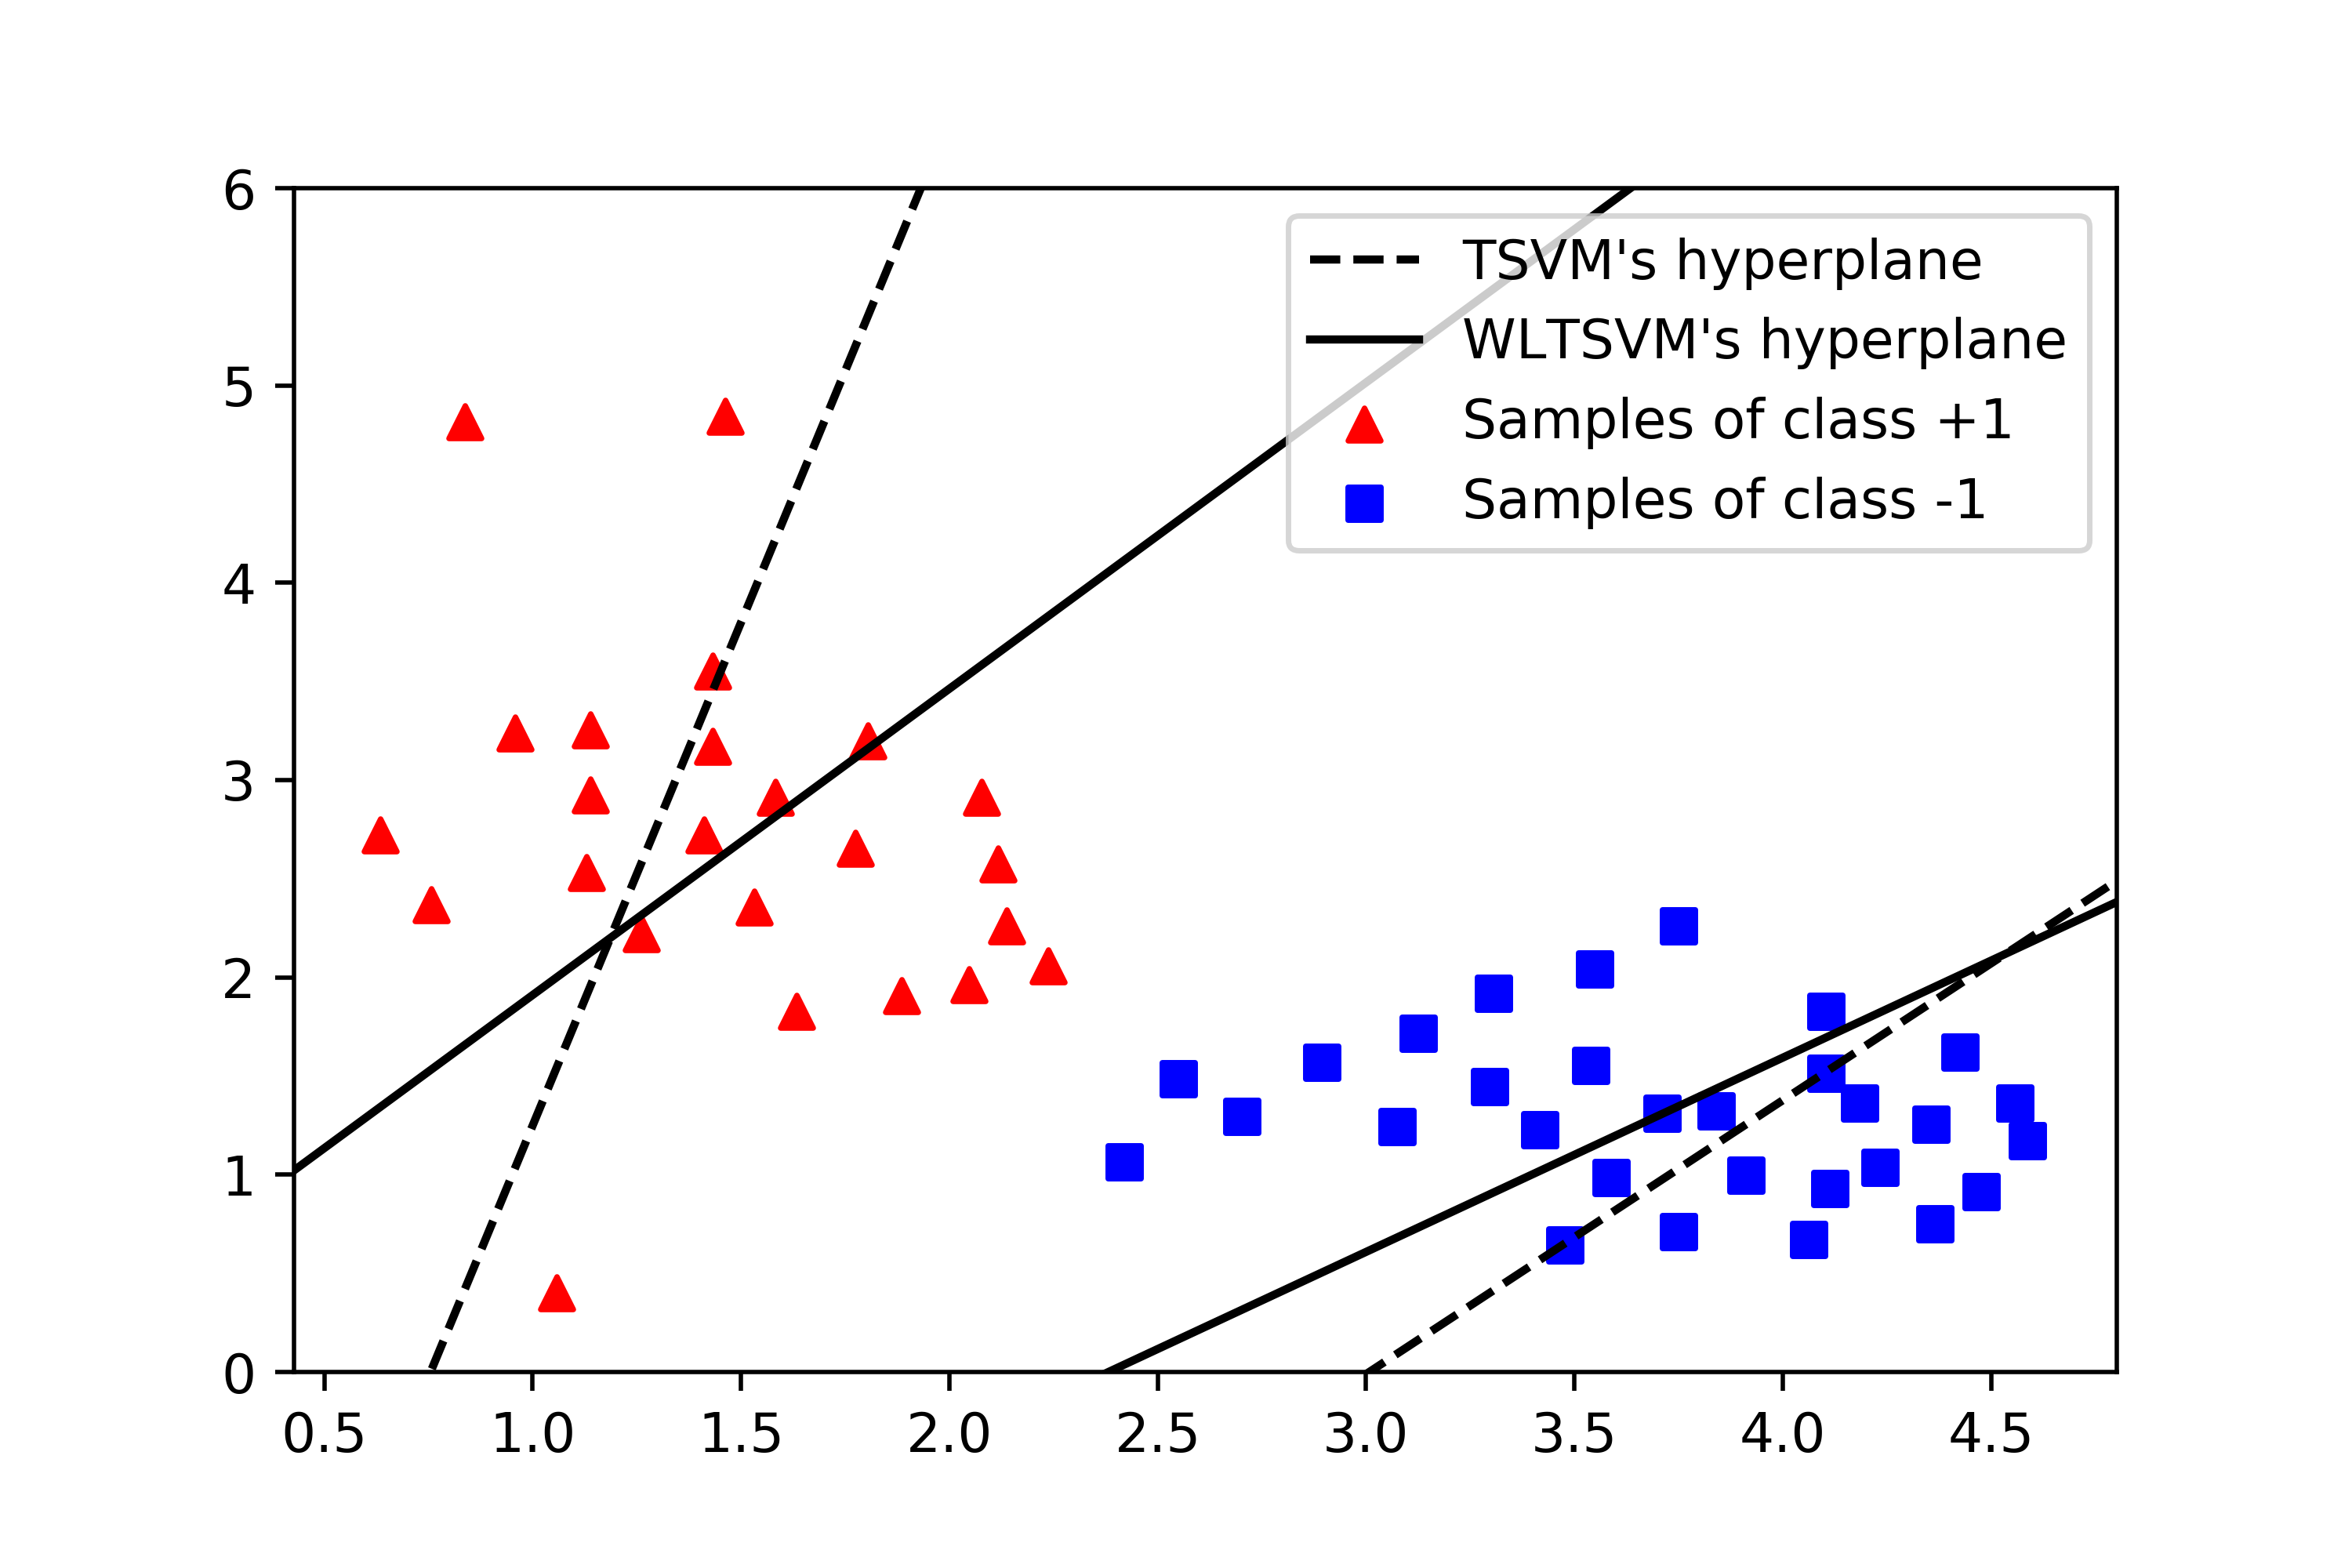
\includegraphics[scale=0.5]{TSVM-vs-WLTSVM}
	\caption{مقایسه هندسی روش \lr{WLTSVM} با روش \lr{TSVM} }
	\label{fig:TSVM-WLTSVM}
\end{figure}

همانطور که شکل ‏\ref{fig:TSVM-WLTSVM} در نشان داده شده است، ابرصفحه غیرموازی در روش \lr{WLTSVM} به نمونه‌های پرتراکم نزدیک‌تر و از نمونه‌های پرت فاصله بیشتری دارد. در این روش دو مسئله بهینه‌سازی اصلی به صورت زیر تعریف می‌شود.
\begin{equation}
\begin{split}
\mathop{{ min}}\limits_{w_{1} ,b_{1}} \qquad & \frac{1}{2}\sum\limits_{i=1}^{m_{1}}{\sum\limits_{j=1}^{m_{1}}{W^{(1)}_{s,ij}(w^{T}_{1}x^{(1)}_{j}+b_{1})^{2}}}+c\sum\limits_{j=1}^{m_{2}}\xi_j \\
\textrm{\lr{s.t. }} \qquad & -f^{(2)}_{j}(w^{T}_{1}x^{(2)}_{j}+b_{1})+\xi_{j} \ge f^{(2)}_{j} \\
& \xi_{j} \ge 0,\quad j=1,...,m_{2}
\end{split}
\label{eq:56}
\end{equation}
\begin{equation}
\begin{split}
\mathop{{ min}}\limits_{w_{2} ,b_{2}} \qquad & \frac{1}{2}\sum\limits_{i=1}^{m_{2}}{\sum\limits_{j=1}^{m_{2}}{W^{(2)}_{s,ij}(w^{T}_{2}x^{(2)}_{j}+b_{2})^{2}}}+c\sum\limits_{j=1}^{m_{1}}\eta_j \\
\textrm{\lr{s.t. }} \qquad & f^{(1)}_{j}(w^{T}_{2}x^{(1)}_{j}+b_{2})+\eta_{j} \ge f^{(1)}_{j} \\
& \eta_{j} \ge 0,\quad j=1,...,m_{2}
\end{split}
\label{eq:57}
\end{equation}
در روابط \ref{eq:56} و \ref{eq:57}،  $c$ پارامتر خطا،  $\xi$ و $\eta$ متغیر لغزش،  $W_{s,ij}^{(1)}$ و  $W_{s,ij}^{(2)}$ به ترتیب نشان دهنده گراف درون کلاسی کلاس مثبت و منفی است. همچنین  $f_{j}^{(1)}$ و $f_{j}^{(2)}$ به ترتیب بیانگر نمونه‌های حاشیه‌ای کلاس مثبت و منفی است. در اینجا نکته حائز اهمیت این است که در قید مسئله بهینه‌سازی فقط نمونه‌های حاشیه‌ای کلاس مقابل در نظر گرفته می‌شود. در حالی که در روش \lr{TSVM} اصلی، تمام نمونه‌های کلاس مقابل در قید مسئله بهینه‌سازی لحاظ شده است. در نتیجه با در نظر گرفتن نمونه‌های حاشیه‌ای، مرتبه زمانی روش \lr{WLTSVM} نسبت به \lr{TSVM} کاهش می‌یابد.

با استفاده از تابع لاگرانژ و شرایط \lr{KKT} حالت دوگان مسئله اصلی \ref{eq:56} و \ref{eq:57} در زیر تعریف شده است.
\begin{equation}
\begin{split}
\mathop{{ min}}\limits_{\alpha} \qquad & \frac{1}{2}{{\alpha }^{T}}(F^{T}G){{({{H}^{T}}DH)}^{-1}}{({G}^{T}F)}\alpha -e_{2}^{T}F\alpha  \\
\textrm{\lr{s.t. }} \qquad & 0{{e}_{2}}\le \alpha \le {{c}}{{e}_{2}}
\end{split}
\label{eq:58}
\end{equation}
\begin{equation}
\begin{split}
\mathop{{ min}}\limits_{\beta} \qquad & \frac{1}{2}{{\beta }^{T}}(P^{T}H){{({{G}^{T}}QG)}^{-1}}{({H}^{T}P)}\beta -e_{1}^{T}P\beta  \\
\textrm{\lr{s.t. }} \qquad & 0{{e}_{1}}\le \beta \le {{c}}{{e}_{1}}
\end{split}
\label{eq:59}
\end{equation}

در رابطه \ref{eq:58} و \ref{eq:59}،  $D=diag(d^{(1)}_{1},d^{(1)}_{2},\dots,d^{(1)}_{m_{1}})$ و  $Q=diag(d^{(2)}_{1},d^{(2)}_{2},\dots,d^{(2)}_{m_{2}})$ نشان دهنده ماتریس وزن کلاس مثبت و منفی است.  همچنین  $P=diag(f^{(1)}_{1},f^{(1)}_{2},\dots,f^{(1)}_{m_{1}})$  و $F=diag(f^{(2)}_{1},f^{(2)}_{2},\dots,f^{(2)}_{m_{2}})$ نشان دهنده نمونه‌های حاشیه‌ای کلاس مثبت و منفی است. بعد از حل کردن مسئله بهینه‌سازی دوگان، مدل خروجی با حل کردن روابط زیر بدست می‌آید.
\begin{equation}
\left[ \begin{aligned}
& {{w}_{1}} \\
& {{b}_{1}} \\
\end{aligned}\right]= -{{({{H}^{T}}DH)}^{-1}}{{G}^{T}}F\alpha
\label{eq:60}
\end{equation}
\begin{equation}
\left[ \begin{aligned}
& {{w}_{2}} \\
& {{b}_{2}} \\
\end{aligned}\right]= {{({{G}^{T}}QG)}^{-1}}{{H}^{T}}P\beta
\label{eq:61}
\end{equation}

نسخه غیر خطی روش \lr{WLTSVM} در مقاله اصلی شرح داده شده است \cite{ye2012}. روش \lr{WLTSVM} نسبت به \lr{TSVM} اصلی برتری‌های نظیر دقت دسته‌بندی بیشتر و مرتبه‌زمانی بهتر را دارد. با این حال روش \lr{WLTSVM} دارای نقاط ضعفی است که عبارتند از:
\begin{enumerate}
	\item روش  \lr{WLTSVM}به هر نمونه بر اساس تعداد نزدیک‌ترین همسایه‌هایش وزن نسبت می‌دهد. به عنوان مثال، وزن نمونه‌های کلاس مثبت از طریق رابطه زیر محاسبه می‌شود.
	\begin{equation}
	{{d}_{j}^{(1)}}=~\underset{i=1}{\overset{{{m}_{1}}}{\mathop \sum }}\,{{W}_{s,ij}}~,~j=1,2,\ldots ,{{m}_{1}}
	\label{eq:62}
	\end{equation}
	در رابطه \ref{eq:62}، متغیر $d_{j}^{(1)}$ نشان دهنده وزن نمونه $x_{j}$ است و  $W_{s,ij}$ مقدار 0 یا 1 دارد. در حالی که می‌توان به همسایه‌های یک نمونه مقداری بین 0 تا 1 براساس فاصله شان نسبت داد. 
	
	\item این روش نیز مانند \lr{TSVM} ریسک تجربی را در مسائل اصلی \ref{eq:56} و \ref{eq:57} کمینه می‌کند. بطوریکه برای جلوگیری از شرایط ماتریس منفرد، معکوس ماتریس‌های   $({H}^{T}DH)^{-1}$ و  $({G}^{T}QG)^{-1}$  به ترتیب با   $({H}^{T}DH + \varepsilon I)^{-1}$ و $({G}^{T}QG + \varepsilon I)^{-1}$  جایگزین میشود. بنابراین تنها راه حل تقریبی مسائل \ref{eq:58} و \ref{eq:59} بدست می‌آید.
	\item با وجود اینکه روش  \lr{WLTSVM} مرتبه زمانی را با لحاظ کردن نمونه‌های حاشیه‌ای در قید مسئله بهینه‌سازی کاهش می‌دهد. در این روش، \lr{k} تا از نزدیک‌ترین همسایه‌های تمام نمونه‌های آموزشی باید محاسبه شود. بنابراین پیچیدگی محاسباتی کلی این روش برابر با  $\mathcal{O}(2m_{1}^{3}+m^{2}logm)$ است. با فرض اینکه  $m_{1}=m_{2}$  و  $m_{1},m_{2} \ll m$. روش‌های جدید و سریع \lr{KNN} برای حل کردن این مشکل می‌تواند استفاده شود.
\end{enumerate}

\subsubsection{سایر گسترش‌های ماشین بردار پشتیبان دو قلو}\label{sec:2:2:3:4}
در این زیربخش، سایر روش‌های مبتنی بر \lr{TSVM} به طور خلاصه معرفی می‌شود. هر کدام از این از گسترش ها، یک نقطه ضعف روش \lr{TSVM} را حل کرده‌اند \cite{ding2014,ding2017,huang2018}. در سال 2013، ماشین بردار پشتیبان دو قلو ساختاری  \footnote{\lr{Structural Twin Support Vector Machine (STSVM)}}(\lr{STSVM}) ارائه گردید \cite{qi2013}.  این روش یادگیری اطلاعات مفید ساختاری درون هر کلاس و توزیع نمونه‌ها را از طریق خوشه‌بندی سلسله مراتبی در مدل خروجی لحاظ می‌کند.  

در سال 2014، ماشین بردار پشتیبان دو قلو مبتنی بر انرژی\footnote{\lr{Energy-based Model of Least Squares Twin Support Vector Machine (ELS-TSVM)}}  (\lr{ELS-TSVM}) ارائه شد \cite{nasiri2014}. در این روش، پارامتر انرژی برای دو ابرصفحه غیرموازی تعریف شده است. بطوریکه مقدار این پارامتر باتوجه به دانش قبلی تعیین می‌شود تا اثر نمونه‌های نویزی و پرت کاهش یابد. در سال 2015، ماشین بردار پشتیبان دو قلو ساختاری با رویکرد گراف نزدیک‌ترین همسایه (\lr{KNN-STSVM}) معرفی شد \cite{pan2015}. در این روش، علاوه بر در نظر گرفتن اطلاعات ساختاری نمونه‌ها، با استفاده از گراف نزدیک‌ترین همسایه به نمونه‌ها وزن داده می‌شود. در نتیجه، دقت مدل خروجی افزایش می‌یابد.

در سال 2016، ماشین بردار پشتیبان دو قلو چند کلاسه با رویکرد مبتنی بر نزدیک‌ترین همسایه\footnote{\lr{ K-nearest neighbor-based weighted multi-class twin support vector machine (KWM-TSVM)}}  (\lr{KWM-TSVM}) معرفی شد \cite{xu2016}. این روش با استفاده از گراف نزدیک‌ترین همسایه، اطلاعات درون کلاسی و برون کلاسی را در تابع هدف مسئله بهینه‌سازی لحاظ می‌کند. در نتیجه پیچیدگی زمانی و دقت مدل بهبود یافته است. در سال 2018، یک روش امن برای کاهش تعداد نمونه‌ها\footnote{\lr{Safe instance reduction rule}}  در روش \lr{KWM-TSVM } ارائه گردید \cite{pang2018}. این روش بخش زیادی از نمونه‌های دو کلاس را قبل از آموزش مدل حذف می‌کند. بنابراین پیچیدگی محاسباتی به طور قابل توجه‌ای کاهش یافته است. 

\begin{table}
	\small
	\centering
	\caption{مرور کلی گسترش‌های مبتنی بر روش  \lr{TSVM}}
	
	\begin{tabular}{c c p{8cm}}
		\hline
		روش یادگیری & سال معرفی & \multicolumn{1}{c}{ایده اصلی} \\
		\hline
		\lr{LS-TSVM} \cite{kumar2009} & 2009 & حل دستگاه معادلات خطی به جای مسئله دوگان که باعث افزایش چشم‌گیر سرعت یادگیری شده است. \\
		\lr{TBSVM} \cite{shao2011} & 2011 & ریسک ساختاری را در مسئله بهینه‌سازی خود کمینه می‌کند. همچنین از شرایط ماتریس منفرد جلوگیری می‌کند. \\
		\lr{WLTSVM} \cite{ye2012} & 2012 & با استفاده از گراف نزدیک‌ترین همسایه به هر نمونه وزن می‌دهد و نمونه‌های حاشیه‌ای هر کلاس را مشخص می‌کند. \\
		\lr{STSVM} \cite{qi2013} & 2013 & اطلاعات ساختاری را از طریق خوشه‌بندی سلسله مراتبی در مدل خروجی لحاظ می‌کند. \\
		\lr{ELS-TSVM} \cite{nasiri2014} & 2014 & پارامتر انرژی برای دو ابرصفحه معرفی شده است که اثر نمونه‌های نویزی و پرت را در مدل خروجی کمتر می‌کند. \\
		\lr{KNN-STSVM} \cite{pan2015} & 2015 & اطلاعات ساختاری با گراف نزدیک‌ترین همسایه برای بهبود دقت مدل خروجی ترکیب شده است. \\
		\lr{KWM-TSVM} \cite{xu2016} & 2016 & روش \lr{TSVM} چندکلاسه را با استفاده از گراف نزدیک‌ترین همسایه از تظر دقت و پیچیدگی زمانی بهبود داده است. \\
		\lr{SIR-KMTSVM} \cite{pang2018} & 2018 & بخش زیادی از نمونه‌های دو کلاس را با استفاده از یک قاعده امن حذف می‌کند. بطوریکه پیچیدگی زمانی روش \lr{TSVM} چند کلاسه بهبود یافته است. \\
		\hline
	\end{tabular}
\label{tab:2:1}
\end{table}
